\documentclass{article}

\usepackage{defines}

\begin{document}

\tickettitle{6}{Понятие аффинного пространства. Аффинные системы координат. Прямая в аффинном пространстве. Декартовая прямоугольная система координат. Теорема о геометрическом смысле декартовых координат на прямой.}

\define{аффинного пространства}

Аффинное пространство $\A$ --- множество элементов (точек), которому сопоставлены:
\begin{enumerate}
	\item{}Линеал $L$, называемый присоединённым к $\A$
	\item{}Правило, по которому $(\forall A,B\in\A)\;\exists\lvec{AB}\in L$
	\item{}Аксиомы:
	\begin{enumerate}[label=\Roman*.]
		\item{}\tikzmark{6:ax_1}$(\forall \vec{a},\vec{b}\in L)\;\vec{a}+\vec{b}=\vec{b}+\vec{a}$
		\item{}$(\forall \vec{a},\vec{b},\vec{c}\in L)\;(\vec{a}+\vec{b})+\vec{c}=\vec{a}+(\vec{b}+\vec{c})$
		\item{}$\exists \vec{0}\in L:(\forall \vec{a}\in L)\;\vec{a}+\vec{0}=\vec{a}$
		\item{}$(\forall \vec{a}\in L)\;\exists \vec{b}\in L:\vec{a}+\vec{b}=\vec{0}$
		\item{}$(\forall \vec{a}\in L,\lambda, \mu\in\R)\;\lambda(\mu\vec{a})=(\lambda\mu)\vec{a}$
		\item{}$(\forall \vec{a}\in L,\lambda,\mu\in\R)\;(\lambda+\mu)\vec{a}=\lambda\vec{a}+\mu\vec{a}$
		\item{}$(\forall \vec{a},\vec{b}\in L,\lambda\in\R)\;\lambda(\vec{a}+\vec{b})=\lambda\vec{a}+\lambda\vec{b}$
		\item{}\tikzmark{6:ax_8}$(\forall \vec{a}\in L)\;1\cdot\vec{a}=\vec{a}$

		\item{}$L$ --- конечномерен
		\item{}$(\forall A\in\A,\vec{v}\in L)\;\exists B\in\A:\lvec{AB}=\vec{v}$
		\item{}$(\forall A,B,C\in\A)\;\lvec{AB}+\lvec{BC}=\lvec{AC}$
	\end{enumerate}
\end{enumerate}

$\dim\A:=\dim L=n$, $\A=\A^{n}$
\begin{tikzpicture}[remember picture, overlay]
	\draw [decorate, decoration={brace}] ($({pic cs:6:ax_1}) + (17em, 1em)$) -- ($({pic cs:6:ax_8}) + (17em,0)$)
	node [midway, right] {Акисомы линеала $L$};
\end{tikzpicture}

\define{аффинной системы координат}

Аффинной системой координат $O\vec{e}_1\vec{e}_2...\vec{e}_{n}$ аффинного пространства $\A^{n}$ называется совокупность:
\begin{enumerate}
	\item{}точки $O\in\A^{n}$ --- начала координат
	\item{}$(\vec{e}_1,\vec{e}_2,...,\vec{e}_{n})$ --- базиса присоединённого линеала $L^{n}$
\end{enumerate}

$\vec{r}_A=\lvec{OA}$ --- радиус-вектор точки $A$

\vspace{2em}
\begin{minipage}{0.5\linewidth}
	\centering
	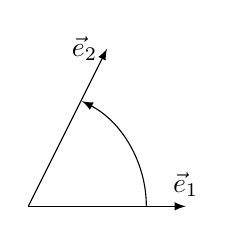
\begin{tikzpicture}
		\draw [-latex] (0,0)--(2,0) node[above] {$\vec{e}_{1}$};
		\draw [-latex] (0,0)--(1,2) node[left] {$\vec{e}_{2}$};
		\draw [-latex] (1.5,0) arc (0:63:1.5);
	\end{tikzpicture}
	\captionof{figure}{Правая система координат}
\end{minipage}%
\begin{minipage}{0.5\linewidth}
	\centering
	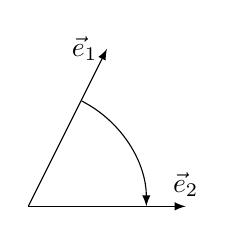
\begin{tikzpicture}
		\draw [-latex] (0,0)--(2,0) node[above] {$\vec{e}_{2}$};
		\draw [-latex] (0,0)--(1,2) node[left] {$\vec{e}_{1}$};
		\draw [latex-] (1.5,0) arc (0:63:1.5);
	\end{tikzpicture}
	\captionof{figure}{Левая система координат}
\end{minipage}

\pagebreak

\define{аффинных координат}

Аффинные координаты $A\in\A$ в системе $O\vec{e}_1\vec{e}_2...\vec{e}_{n}$ --- координаты её радиус-вектора.

Аффинные координаты определяются однозначно, тк разложение радиус-вектора по базису~единственно.

\define{прямой в аффинном пространстве}

Прямой в аффинном пространстве, проходящей через $A_0\in\A$ в направлении $\vec{v}\in L,\;\vec{v}\neq \vec{0}$\\
называется $\setdef{P\in\A}{\exists\lambda\in\R:\lvec{AP}=\lambda\vec{v}}$.

\define{ортонормированного базиса}

Базис $(\vec{e}_1,\vec{e}_2,...,\vec{e}_{n})$ --- ортонормированный, если
$(\forall i=\overline{1,n})\;|\vec{e}_{i}|=1$ $\land$ $(\forall i,j=\overline{1,n}:i\neq j)\;\vec{e}_{i}\perp\vec{e}_{j}$

Понятие перпендикулярности векторов определеяется позже.

\define{декартовой прямоугольной системы координат (ДПСК)}

$O\vec{e}_{1}\vec{e}_{2}...\vec{e}_{n}$ --- ДПСК, если $(e_{i})$ --- ортонормированный.

\define{алгебраической меры}

$\lambda$ --- алгебраическая мера $\vec{a}$ на оси, определяемой вектором $\vec{e}_{1}$, если $\vec{a}=\lambda\vec{e}_{1}$.

$\mes_{\vec{e}_{1}}\vec{a}:=\lambda$

\theorem

Координаты $A\in\A^{1}$ относительно $O\vec{e}_{1}$ --- $\mes_{\vec{e}_{1}}\lvec{OA}$.

\proof
\begin{align*}
	\lambda\text{ --- координаты $A$}\Rarr\vec{r}_{A}=\lvec{OA}=\lambda\vec{e}_{1}\Rarr\lambda=\mes_{\vec{e}_{1}}\lvec{OA}\qed
\end{align*}
\end{document}
